\documentclass[11pt]{article}
\usepackage{amssymb,amsmath,graphicx}    % needed for including graphics e.g. EPS, PS
\usepackage[hmargin=2cm,vmargin=2cm]{geometry}
\graphicspath{{./img/}}
%\usepackage{amssymb,amsmath,amsthm,graphicx,setspace,hyperref}
%\topmargin -1.5cm        % read Lamport p.163
%\oddsidemargin -0.04cm   % read Lamport p.163
%\evensidemargin -0.04cm  % same as oddsidemargin but for left-hand pages
%\textwidth 16.59cm
%\textheight 21.94cm 
%pagestyle{empty}       % Uncomment if don't want page numbers
\parskip 7.2pt           % sets spacing between paragraphs
%\renewcommand{\baselinestretch}{1.5} % Uncomment for 1.5 spacing between lines
\parindent 0pt		 % sets leading space for paragraphs
\numberwithin{equation}{section}	%Puts equation numbers in the form of m.n

\begin{document}         
\title{ECE 795: Quantitative Electrophysiology\\Project}
\author{Philip Chrapka}
\date{January 11, 2010}
\maketitle
% Start your text

The electromyographic (EMG) signal is a very complex signal that can provide information about the activation of skeletal muscles. It is a linear combination of the motor unit action potentials that activate these muscles \cite{Beck2005,Jaskolska2006}. The literature shows many cases where information can be extracted from an EMG signal relating to all aspects of muscle function. A common and well established relationship is that between the amplitude of the surface EMG and the amount of force produced by the muscle, where a greater amplitude reflects a larger force \cite{Beck2005}. However, there are many factors that can affect an EMG signal including the force of contraction, interelectrode spacing, the type of muscle under scrutiny, etc.

This project explores a few variable parameters when acquiring EMG data from the biceps brachii (BB). Additionally, the data is analyzed to explore what relationships, between the EMG signal and the experimental parameters, can be portrayed by signal statistics.

The raw EMG data was collected using the Clevemed data acquisition system following the protocol described in the project outline. The collected EMG data was post processed in MATLAB. Depending on the requirements for each section, the root mean squared (RMS) value as well as the power spectrum were determined. The RMS value was calculated according to the following formula:
\begin{gather}
\textrm{Root Mean Squared} = \sqrt{\frac{1}{n}\sum_n{x^2(t)}} \nonumber
\end{gather}
where \(x(t)\) is the raw EMG signal. The power spectrum was calculated using Welch's periodogram using the default values in MATLAB (ie. 8 windows). In order to describe the power spectrum, the centroid frequency was determined using the following formula:
\begin{gather}
\textrm{Centroid Frequency} = \frac{\sum_{n=0}^{N-1}{f(n)x(n)}}{\sum_{n=0}^{N-1}{x(n)}} \nonumber
\end{gather}
where \(f(n)\) represents the frequency and \(x(n)\) represents the weight or power of that frequency.

It should be noted that for questions 1, 2 and 4, some of the raw EMG data contained a wandering baseline (possibly indicating motion artefacts), therefore it was first filtered through a band pass filter from 20Hz to 250Hz using a \(60^\textrm{th}\) order Chebyshev filter. This resulted in more realistic RMS values. In addition, this filtering removed a large amount of power in the lower frequency range (0-2 Hz) which probably represented some DC component present in the signal. This is acceptable since this portion of the signal would not have originated from the muscle and would have otherwise affected the centroid frequency. 

% Joint angles
\section*{Question 1}
The first parameter that was investigated was the elbow joint angle during an isometric contraction, which involves holding a 5 pound weight for over 10 seconds at a specified angle. As the elbow joint angle decreases, the BB shortens and contracts. By varying the elbow joint angle, the EMG data describes the activity of the BB at different stages of contraction. 

Five joint angles were investigated: \(60^\circ\), \(90^\circ\), \(120^\circ\), \(135^\circ\) and \(150^\circ\), where full extension corresponds to \(180^\circ\). The analysis was performed on 10 seconds of raw EMG data and the MATLAB code can be seen in ques1.m. Figure \ref{fig1a} shows the raw EMG and power spectrum for a joint angle of \(60^{\circ}\). The results of the analysis for different joint angles can be seen in Figure \ref{fig1b}. 

% fig1a
\begin{figure}[!ht]
  \centering
    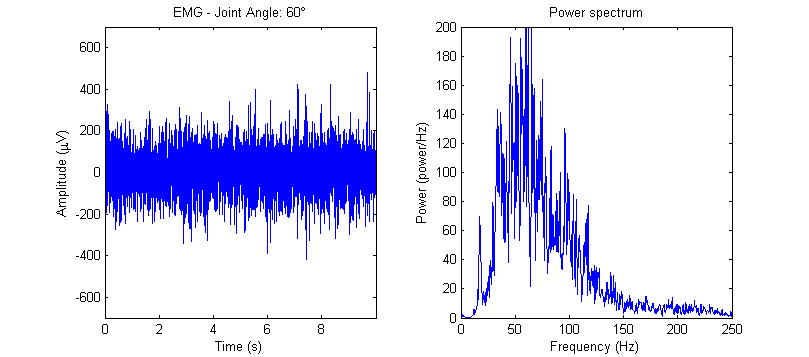
\includegraphics[width=0.75\textwidth]{fig1a}
	\caption{Raw EMG data and power spectrum for a joint angle of \(60^{\circ}\)}
	\label{fig1a}
\end{figure}
% fig1b
\begin{figure}[!ht]
  \centering
    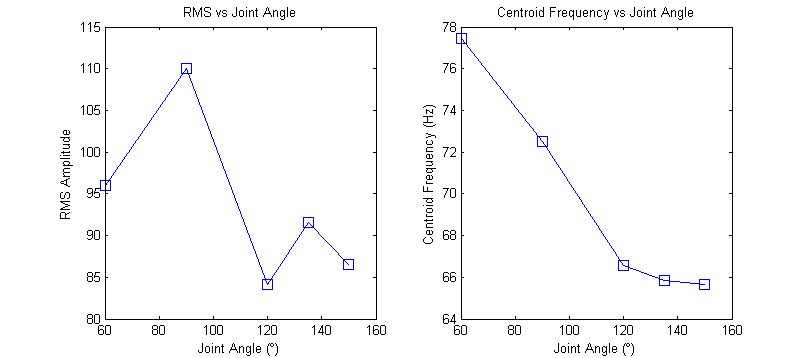
\includegraphics[width=0.75\textwidth]{fig1b}
	\caption{RMS and Centroid Frequency vs Joint Angle}
	\label{fig1b}
\end{figure}

The results in Figure \ref{fig1b} clearly show that the RMS value seems to peak at an elbow angle of \(90^\circ\) and then decrease for angles larger and smaller. In my opinion, the peak at \(90^\circ\) makes intuitive sense since it is at this point that the BB has to counteract the greatest force of gravity. However, predicting the amount of force that will be exerted by the BB to counteract the dumbbell is difficult, due to the complexity of the anatomy of the upper limb. 

The literature also seems to have difficulty demonstrating the relationship between RMS and elbow angle. A study comparing EMG data while varying elbow joint angles during isometric contractions shows a complex relationship \cite{Mamaghani2002}. At 20\%, 40\% and 60\% of the subjects' maximum voluntary contraction (MVC) an elbow angle of \(120^\circ\) displayed the highest RMS value. At 20\% and 40\% of MVC an elbow angle of \(60^\circ\) showed a higher RMS value than that of \(90^\circ\). Whereas, at 60\% of MVC an elbow angle of \(90^\circ\) showed a higher RMS value than that of \(60^\circ\). 

Another study comparing EMG responses in young and old women, shows that the RMS value increases with a smaller elbow joint angle \cite{Jaskolska2006}. This finding agrees with my results as the RMS value at a \(60^\circ\) joint angle is higher than the RMS for joint angles \(\geq 120^\circ\). When the muscle shortens it deforms and the electrodes may be oriented differently with respect to the sources that they are measuring \cite{Jaskolska2006}. 

A third study using a measure of average EMG shows almost the same pattern as my results \cite{Linnamo2006}. It shows that the overall average EMG of the BB decreases with increasing elbow angle but peaks around \(90^\circ\).

Figure \ref{fig1b} also shows a clear relationship where the centroid frequency decreases with increasing elbow joint angle. This result matches the literature quite well \cite{Mamaghani2002}. I was unable to find an explanation of this result in the literature. The centroid frequency is related to the conduction velocity of muscle fibers \cite{Arendt-Nielsen1989}. Therefore, it could be said that the elbow joint angle influences what types of motor units are recruited to perform the isometric contraction.

%\clearpage

% Electrode position
\section*{Question 2}
The second parameter that is investigated is the interelectrode spacing (IES). The distance between electrodes is important because it determines what part of the muscle is measured. A larger IES would encompass a larger portion of the muscle and give a better picture of the activity of the majority of the muscle \cite{Beck2005}. On the other hand, a larger IES would be susceptible to cross-talk from other muscles \cite{Beck2005}. Using a simulated model, another paper reported that increasing IES increased the distance from which EMG signals could be detected \cite{Fuglevand1992}. Theoretically, since the EMG would have more sources to detect at a larger IES, the RMS value should be larger \cite{Beck2005, Alemu2003}. As for the centroid frequency, it has a tendency to decay as the IES becomes larger however the difference is not statistically significant \cite{Beck2005}. 

The interelectrode spacings that were used for this portion were: 3 mm, 3.6 mm, 4.2 mm, 4.8 mm and 6 mm. At each spacing, a 5 pound weight was held at an angle of \(90^\circ\) for about 10 seconds. The analysis was performed using 5 seconds of data and the code can be seen in ques2.m. A sample of the output from the analysis can be seen in Figure \ref{fig2a}.

% fig2a
\begin{figure}[!ht]
  \centering
    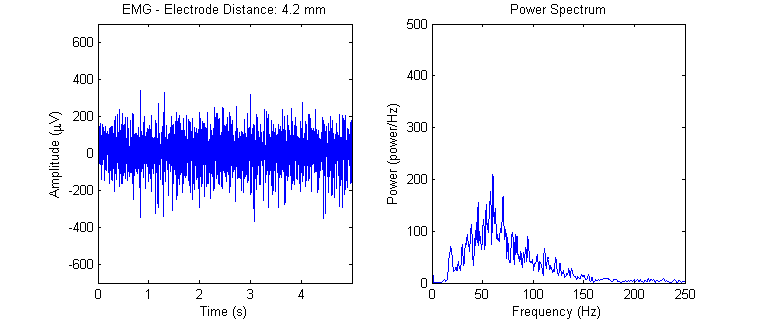
\includegraphics[width=0.75\textwidth]{fig2a}
	\caption{Raw EMG data and power spectrum for an interelectrode spacing of 4.2 mm}
	\label{fig2a}
\end{figure}
% fig2b
\begin{figure}[!ht]
  \centering
    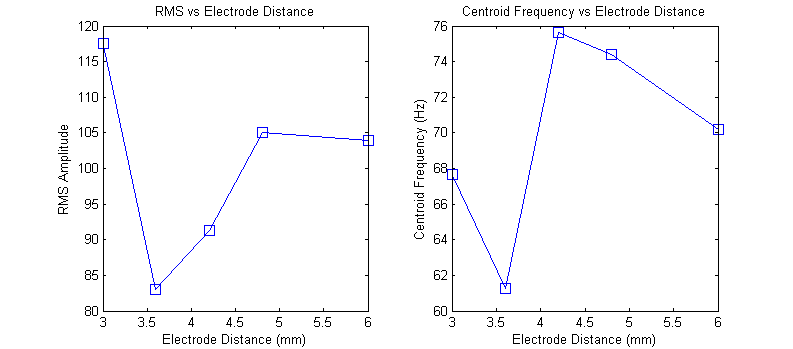
\includegraphics[width=0.75\textwidth]{fig2b}
	\caption{RMS and Centroid Frequency vs Interelectrode spacing}
	\label{fig2b}
\end{figure}

The final results for all interelectrode spacings can be seen in Figure \ref{fig2b}. The RMS results tend to increase with increasing IES as the literature suggests, with the exception of the first data point. It could be possible that the results could have been affected by the re-application and removal of the electrodes, since only one set of electrodes was used throughout the entire experiment. This could have caused the EMG signal recorded at 3 mm to be much stronger because of better adhesion of the electrodes. For larger IES, the centroid frequency tends to follow a decreasing pattern with increasing IES. It does, however, contain a strange jump between 3.6 and 4.2 mm. The differences in centroid frequency between my results and those reported in the literature could possibly be excused by the fact that my sample size contains only one individual. One individual could skew the results and would not necessarily represent the average case. This fact should also be taken into consideration for the other sections of this project.

%\clearpage

% Motion artefact
\section*{Question 3}
Motion artefacts in an EMG signal can become a serious issue when studying a moving subject. They are caused by movement at the skin electrode interface \cite{DeLuca2010}. The artefacts can originate from the movement of a muscle during contraction as well as the movement of a force impulse traveling through the muscle \cite{DeLuca2010}. It has been reported that motion artefacts mainly contaminate the signal at lower frequencies, therefore the most obvious solution is a standard high pass filter \cite{Conforto1999}. However, a disadvantage of this method is the possibility of phase distortion which could affect the timing of the filtered signal \cite{Conforto1999}. Thus, many other methods have been proposed to filter out this artefact including a moving average procedure, a median average procedure or even a wavelet-based procedure \cite{Conforto1999}. To demonstrate the concept of artefact removal and for simplicity, the high pass filter is used in the following analysis. The question that remains is that of which corner frequency should be applied to remove the motion artefact. DeLuca et al. \cite{DeLuca2010} examine various standard corner frequencies that are used for the high pass filter and conclude that 20 Hz offers the best compromise.

The analysis for this question was slightly modified. For an accurate comparison, both EMG signals in Figures \ref{fig3emg} and \ref{fig3spectrum} were filtered to remove the frequencies above 250 Hz. To remove the motion artefacts, the EMG signal was also filtered to remove frequencies below 20 Hz. The corresponding MATLAB code can be seen in ques3.m.

% fig3emg
\begin{figure}[!ht]
  \centering
    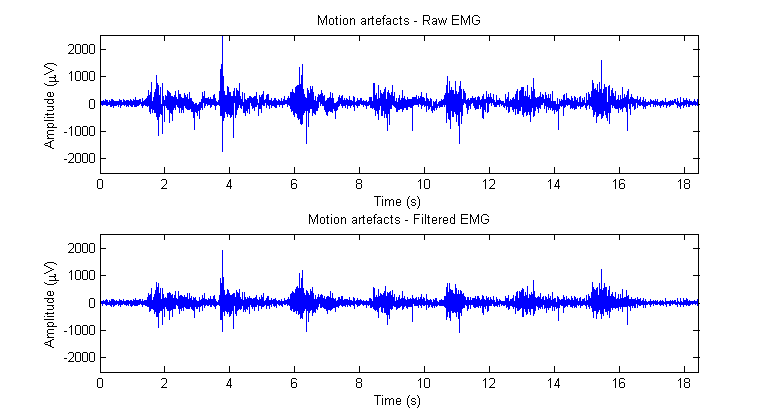
\includegraphics[width=0.75\textwidth]{fig3emg}
	\caption{Raw and filtered EMG signal containing motion artefacts in the time domain}
	\label{fig3emg}
\end{figure}

When comparing Figure \ref{fig3emg} to some of the other sample plots included in this report, it can be seen that the baseline seems to wobble at many points along the signal. It is evident that the signal is affected by the dynamic contraction of the BB. Since the motion artefacts are mainly located in the lower frequency range this would clearly tend to lower the centroid frequency, which is evident in the power spectra, Figure \ref{fig3spectrum}. As we will see in question 4, the centroid frequency is a fairly consistent indication of fatigue within the muscle. Therefore, if the EMG is being relied on as a diagnostic tool, the state of the muscle could be misrepresented with a simple motion artefact.

% fig3spectrum
\begin{figure}[!ht]
  \centering
    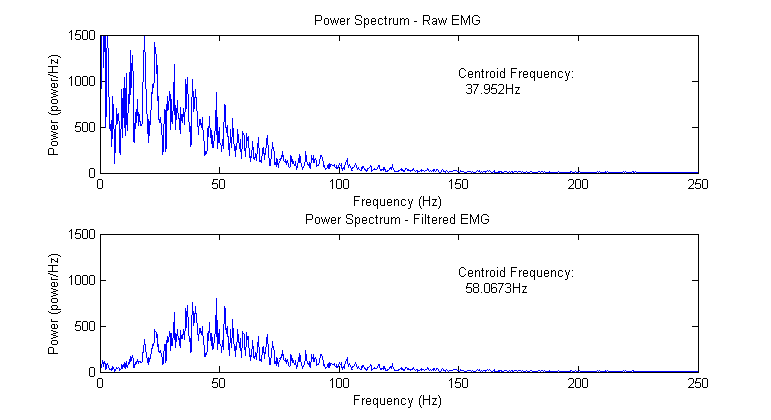
\includegraphics[width=0.75\textwidth]{fig3spectrum}
	\caption{Power spectra of the raw and filtered EMG signal}
	\label{fig3spectrum}
\end{figure}

%\clearpage

% Fatigue
\section*{Question 4}
The goal of this portion of the experiment was to explore muscle fatigue. It required holding a 15 pound weight with an elbow angle of \(90^\circ\) for as long as possible. The amount of data collected was just over 90 seconds. An initial observation of the signal in Figure \ref{fig4a} shows an increase in the amplitude of the EMG signal as the duration of the contraction increases. 

% fig4a
\begin{figure}[!ht]
  \centering
    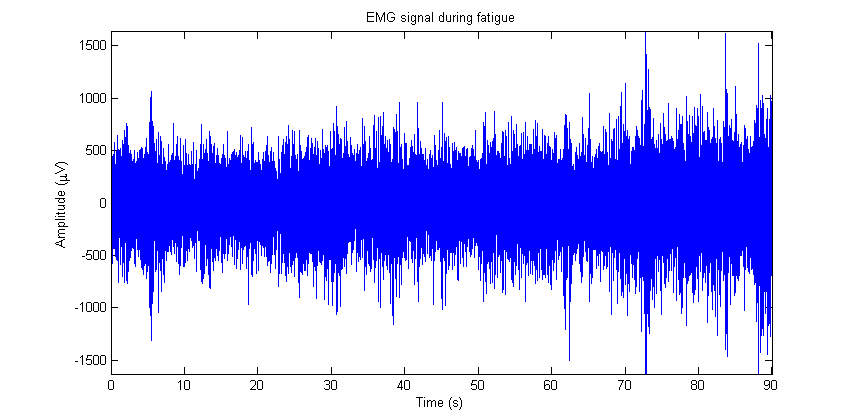
\includegraphics[width=0.75\textwidth]{fig4a}
	\caption{The entire EMG signal in the time domain}
	\label{fig4a}
\end{figure}

The 90 seconds of data was first split into 5 second epochs and the analysis was performed on each 5 second epoch. The MATLAB code can be seen in ques4.m and a sample result can be seen in Figure \ref{fig4b}.

% fig4b
\begin{figure}[!ht]
  \centering
    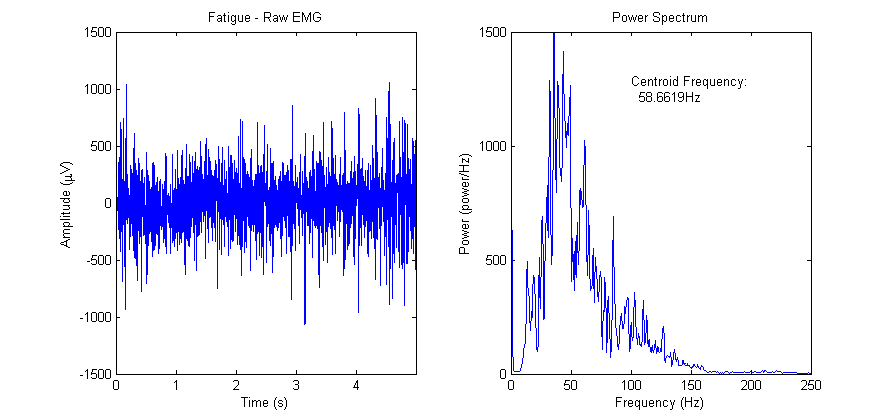
\includegraphics[width=0.75\textwidth]{fig4b}
	\caption{Raw EMG data and power spectrum for one of the 5s epochs}
	\label{fig4b}
\end{figure}

The changes in the power spectrum of an EMG signal is a combination of the effects of a number of different factors including an increase or decrease in the firing rates of motor units, shortening of muscle fibers, conduction velocity, etc. \cite{Arendt-Nielsen1989}. During fatigue, it is known that the power spectrum tends to shift towards the lower frequencies \cite{Arendt-Nielsen1989,Hagg1992,Bigard2001,Sbriccoli2003}. This is best described by the centroid frequency which characterizes the mean of the power spectrum. This shift is mainly attributed to a decrease in the conduction velocity of muscle fibers \cite{Arendt-Nielsen1989}. Figure \ref{fig4c} clearly confirms this fact, where it can be seen that the centroid frequency decreases as the duration of the contraction increases.

% fig4c
\begin{figure}[!ht]
  \centering
    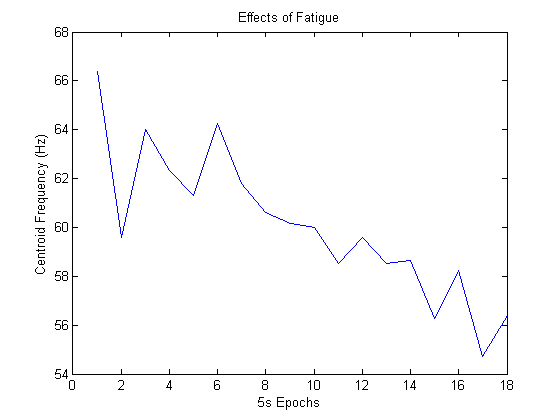
\includegraphics[width=0.75\textwidth]{fig4c}
	\caption{Effect of fatigue on centroid frequency}
	\label{fig4c}
\end{figure}

\clearpage

\bibliographystyle{ieeetr}
\bibliography{sources}

% Stop your text
\end{document}